%!TEX root = ../dokumentation.tex

\chapter{Related Work}\label{cha:RelatedWork}
\section{Existing methods for debugging shaders in the graphics pipeline}
\label{section:debuggingMethods}

For debugging a shader program within the graphics pipeline there are the options to use workarounds to get the values of the variables within the code or to use special drivers provided by the producers of the hardware to get the option to debug on this hardware.

\paragraph{Manual debugging}

The manual way of debugging a shader is by creating outputs of the values within the shader program to see anomalies in their values. This can't be done by writing these values on the console or in a log file like it would be done in a CPU based application because as mentioned in \autoref{section:problems} there is no access to the console or a logger within a shader program. The workaround used here is to return the values projected on the rgba-color values on the resulting image of the program. In this way the programmer can see the rough area in which the values are located on the direct output. The image can also be saved and inspected closer to get the exact values within the pixels of the resulting image.\myCite{Ciardi.2015}

\paragraph{Debugging with special drivers on certain hardware}
\label{section:debuggingMethods_drivers}

It is possible to install special drivers for certain graphics cards provided by their producers to enable debugging of shaders running on this hardware within dedicated environments. The two big suppliers of graphics hardware Nvida and AMD provide these debugging environments in the form of \cite{Nvidia_Nsight} and \cite{AMD_GPUPerfStudio}. These tools can be included into different IDEs or downloaded as standalone applications. There are debugging tools for GPU debugging provided by other sources than the producers of the hardware themselves but for gaining access to the values in the hardware pipeline the drivers of this hardware have to implement specific debugging interfaces.\myCite{Microsoft_debug.2016} Applying these tools enables the use of breakpoints and the inspection of variables within the shader code at runtime\myCite{GLSL_debugger} or dumping the buffer into a file.\myCite{Microsoft_pdb.2019} The disadvantage of this method is that not all graphics cards are supported with such drivers and tools by their producer.

\section{Approaches for debugging compute shaders on the CPU}
\label{section:computeApproaches}

As \myCite{Jukka.2012} states "Relatively little has been published about debugging of GPU programs  in  practice.  Most  of  the  best  practice  guides  and lessons learned papers discuss GPU programming rather than debugging. Although exceptions exist". Among these exceptions are approaches to write compute shaders in other programming languages so that the version of the shader in the other language can be run on the CPU where it can be debugged. This version of the shader will then be translated to the actual shader language so it can run on the GPU with the full performance advantage. This enables the use of all tools the chosen language supports to aid debugging without depending on specific hardware or drivers.

The advantage compute shaders have in comparison with other kinds of shader programs is that they run independently of the graphics pipeline. They are executed by passing inputs and receiving the outputs like any method or program in regular CPU based languages. In the graphics pipeline some of the inputs and outputs would be handled by automated steps of the pipeline. The main difference between CPU based languages and GPU based languages is that for the shaders passing inputs and receiving the output is done by writing into and reading from buffers.

There are projects like \myCite{ILGPU} where a special syntax is required for shaders within the CPU based language to enable the translation of this code as a compute shader to run on the GPU. Switch between running the code on the CPU where it can be debugged and running it on the GPU with optimal performance can be handled within the program.

Other projects like \myCite{Campy} provide a compiler translating the full codebase to run as a compute shader on the GPU. Here it is possible to write the code in the familiar language without having to adapt special syntax rules. To debug the code, it is run within a regular compiler for the language while it will run on the GPU when it is executed with the special compiler.

\section{Translating shaders from other languages}\label{section:translating}

To run code on the GPU usually the programmer has to use one of  multiple low-level languages specialized in this task. To enable programmers to run code on the GPU while being able to stay at the language they are accustomed to there are multiple solutions to translate different languages into these low-level languages.

There are three different types of programming languages. The ones that are directly compiled ahead of time (AOT), the ones that are compiled to an intermediate language which then runs in a JIT(Just in Time) compiler and the ones that are running in an interpreter. For these three types there are different approaches to translate them to a shader language.\myCite{Turton.2017}

For all of these kinds of languages, it is possible to write a compiler translating them directly to the shader language. This is what \myCite{GLSLplusplus} does with the AOT compiled language C++ translating it to the shader language GLSL. In this project created to change the way of writing shader code the possibility of using this to debug the shaders written in C++ is mentioned. \myCite{SharpShader} is another example which uses the Language C\# which is usually compiled to the intermediate language MSIL. In this example C\# code is directly compiled to a Shader languages HLSL or GLSL. In both cases the programmer can use his accustomed language with the limitation of having to write the code for the GPU within special syntax rules to be able to translate it to be translated into a shader for the GPU. An advantage that results of the direct translation is that variable names given in the written code can be retained in the shader code.

Another option with the use of a language that compiles to an intermediate language is to take the code in the intermediate language and further translate it into a shader language. Examples implementing this are \myCite{ILGPU} and \myCite{Campy} where the shaders are written in C\#. This code is then compiled to the intermediate language MSIL. The MSIL code is further translated into the compute language CUDA which then runs on the GPU. Another example is \myCite{SpirvNet} which translates MSIL to Spirv. Spirv is a intermediate language for graphical shader code that can be interpreted as a shader on the GPU or translated further into other shader languages with tools such as \myCite{SPIRVcross} which translates to GLSL. The translation in all of these cases is based on a uniform intermediate language which could be the result of multiple higher level languages. So by writing the translator for this intermediate language the option exists to write the shaders in different languages compilable to this intermediate language. The variable names are lost by compiling to the intermediate language which means that the variable names are not retainable in the shader code.

To get a code translated to a shader code it is also possible to chain multiple existing tools together to translate the language, in which the shaders should be written in, to the desired shader language. An example for this process can be seen in the way the Interpreted language R is translated through multiple steps to run on the GPU in the example "Just-In-Time GPU Compilation for Interpreted Languages with Partial Evaluation" also seen in \autoref{fig:rTranslation}\myCite{Fumero.2017}

\begin{figure}[h!]
  \centering 
  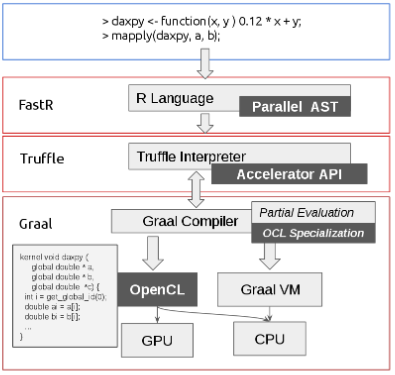
\includegraphics[scale=1]{R_translation.png}
  \caption[Translation order for R to OpenCL \myCite{Fumero.2017}]{"System Overview: Starting from R code our sys-tem transparently generates and executes OpenCL code viaFastR which is built on top of Truffle and Graal." according to \myCite{Fumero.2017}}
  \label{fig:rTranslation}
\end{figure}